%Documento principal do latex para uso no TCC do curso de Sistemas de Informação da Univás.
%Os alunos devem editar apenas os arquivos que estão no diretório "editaveis".
%As figuras que forem utilizadas no TCC devem ser colocadas na pasta "imagens".

%Atenção: Os alunos não devem editar os outros arquivos. Qualquer dúvida procure o professor de TCC e Desenvolvimento de Projetos

\documentclass[a4paper, 12pt, chapter=TITLE, oneside, english, brazil,oldfontcommands]{abntex2}

\usepackage{styles/CodeStyle}           %Formatação de códigos e listagens
\usepackage{styles/EventFlowStyle} %Estilo para o quadro de fluxo de eventos
\usepackage{styles/NuapaStyle}         %Estilo exigido pela Univás

\begin{document} %Início do documento

\pretextual %Início dos Elementos Pré-Textuais


\makeatletter
\renewcommand{\imprimircapa}{%
\begin{capa}%
\begin{center}%
  {\ABNTEXchapterfont\large\MakeUppercase\imprimirautor}\\
  \vspace*{\fill}%
  \vspace*{\fill}%
  \vspace*{\fill}%
  {\ABNTEXchapterfont\bfseries\Large\MakeUppercase\imprimirtitulo}\\
  \vspace*{\fill}%
  {\color{white}%
\abntex@ifnotempty{\imprimirpreambulo}{%
  \hspace{.45\textwidth}
  \begin{minipage}{.5\textwidth}
    \SingleSpacing
    \imprimirpreambulo
  \vspace{.1\textwidth}\\%
  {\imprimirorientadorRotulo:~\imprimirorientador}
  \abntex@ifnotempty{\imprimircoorientador}{%
    \hspace{.45\textwidth}
    {\large\imprimircoorientadorRotulo~\imprimircoorientador}%
  }%
  \end{minipage}%
}%
\color{black}}%
  \vspace*{\fill}\\%
  {\ABNTEXchapterfont\large\bfseries\MakeUppercase\imprimirinstituicao}\\
  {\large\bfseries\MakeUppercase\imprimirlocal}\\
  {\large\bfseries\MakeUppercase\imprimirdata}
\end{center}
\end{capa}
}
\makeatother

\imprimircapa

% folha de rosto 
%\folhaderostoname{Folha de rosto}
%http://code.google.com/p/abntex2/wiki/ComoCustomizar

\makeatletter
\renewcommand{\folhaderostocontent}{
\begin{center}%
  {\ABNTEXchapterfont\large\MakeUppercase\imprimirautor}\\
  \vspace*{\fill}%
  \vspace*{\fill}%
  \vspace*{\fill}%
  {\ABNTEXchapterfont\bfseries\Large\MakeUppercase\imprimirtitulo}\\
  \vspace*{\fill}%
\abntex@ifnotempty{\imprimirpreambulo}{%
  \hspace{.45\textwidth}
  \begin{minipage}{.5\textwidth}
    \SingleSpacing
    \imprimirpreambulo
  \vspace{.1\textwidth}\\%
  {\imprimirorientadorRotulo:~\imprimirorientador}
  \abntex@ifnotempty{\imprimircoorientador}{%
    \hspace{.45\textwidth}
    {\large\imprimircoorientadorRotulo~:\imprimircoorientador}%
  }%
  \end{minipage}%
}%
  \vspace*{\fill}\\%
  {\ABNTEXchapterfont\large\bfseries\MakeUppercase\imprimirinstituicao}\\
  {\large\bfseries\MakeUppercase\imprimirlocal}\\
  {\large\bfseries\MakeUppercase\imprimirdata}
\end{center}
}%end of folhaderostocontent
\makeatother

\imprimirfolhaderosto*{}
\begin{fichacatalografica}
\begin{normalsize}
  \vspace*{\fill}
  % Posição vertical
%  \hrule
  % Linha horizontal
  \begin{center}
  \fbox{
    % Minipage Centralizado
    \begin{minipage}[c]{12.5cm} % Largura
      \vspace{0.7cm}%
      \hspace{0.8cm} \imprimirAutorCitacao ~\\%
      
      \hspace{0.8cm} \imprimirtitulo ~/ \imprimirAutorUm , \imprimirAutorDois ~-- \imprimirlocal: Univás, \imprimirdata. %
      
      \hspace{0.8cm} \pageref{LastPage} f. : il.~\\%
      
      \hspace{0.8cm} \imprimirtipotrabalho~--~\imprimirinstituicao , Univás, \imprimircurso. % 
      
      \hspace{0.8cm} \imprimirorientadorRotulo: ~\imprimirorientador ~\\%

      \hspace{0.8cm} 1. \imprimirPalavraChaveUm. 2. \imprimirPalavraChaveDois. 3. \imprimirPalavraChaveTres. ~ \\%
    \end{minipage}
    }
  \end{center}
\end{normalsize}
\end{fichacatalografica}
\newpage
\setlength{\ABNTEXsignwidth}{10cm}

\begin{folhadeaprovacao}
  \begin{center}
    {\ABNTEXchapterfont\large\MakeUppercase\imprimirautor}\\
    \vspace*{\fill}
    \vspace*{\fill}
    \vspace*{\fill}
    {\ABNTEXchapterfont\bfseries\Large\MakeUppercase\imprimirtitulo}\\
    \vspace*{\fill}
  \end{center}
  Trabalho de conclusão de curso defendido e aprovado em \imprimirDataDaAprovacao ~pela banca examinadora constituída pelos professores:

  ~\newline
  \begin{flushleft}
  \assinatura*{\imprimirorientador \\ \imprimirorientadorRotulo }
  \assinatura*{\imprimirAvaliadorUm \\ \imprimirAvaliadorLabelUm }
  \assinatura*{\imprimirAvaliadorDois \\ \imprimirAvaliadorLabelDois}
  \end{flushleft}
  \vspace*{\fill}
  \vspace*{\fill}
\end{folhadeaprovacao}

\begin{dedicatoria}
\vspace*{\fill}
\vspace*{\fill}
\vspace*{\fill}
\vspace*{\fill}
\vspace*{\fill}
\vspace*{\fill}
De \imprimirAutorUm.
\newline
%início da dedicatória do autor um
Dedico este trabalho \ldots 

\vspace*{\fill}
De \imprimirAutorDois.
\newline
%início da dedicatória do autor dois
Dedico este trabalho \ldots

\end{dedicatoria}

\begin{agradecimentos}

De \imprimirAutorUm
\newline
%início do agradecimento do autor um
\par Agradeço \ldots

\vspace*{\fill}
De \imprimirAutorDois
\newline
%início do agradecimento do autor dois
\par Agradeço \ldots

\end{agradecimentos}





\begin{epigrafe}
\vspace*{\fill}
\begin{flushright}
\textit{‘‘Complicar é simples, \\
simplificar que é complicado.\\
(Paulo Sérgio dos Santos)}
\end{flushright}
\end{epigrafe}

% --- resumo em português ---

\begin{OnehalfSpacing} 

\noindent \imprimirAutorCitacaoMaiuscula. {\bfseries\imprimirtitulo}. {\imprimirdata}.  Monografia -- Curso de {\MakeUppercase\imprimircurso}, {\imprimirinstituicao}, {\imprimirlocal}, {\imprimirdata}.

\vspace{\onelineskip}
\vspace{\onelineskip}
\vspace{\onelineskip}
\vspace{\onelineskip}

\begin{resumo}
~\\
%início do texto do resumo
\noindent Este trabalho apresenta \ldots

%fim do texto do resumo
\vspace{\onelineskip}
\vspace*{\fill}
\noindent \textbf{Palavras-chave}: \imprimirPalavraChaveUm. \imprimirPalavraChaveDois. \imprimirPalavraChaveTres.
\vspace{\onelineskip}
\end{resumo}

\end{OnehalfSpacing}

% --- resumo em inglês ---

\begin{OnehalfSpacing} 

\noindent \imprimirAutorCitacaoMaiuscula. {\bfseries\imprimirtitulo}. {\imprimirdata}.  Monografia -- Curso de {\MakeUppercase\imprimircurso}, {\imprimirinstituicao}, {\imprimirlocal}, {\imprimirdata}.

\vspace{\onelineskip}
\vspace{\onelineskip}
\vspace{\onelineskip}
\vspace{\onelineskip}

\begin{resumo}[Abstract]%
\begin{otherlanguage*}{english}%
\textit{
%início do texto do abstract
\noindent This work presents \ldots
%fim do texto do abstract
}

\vspace{\onelineskip}
\vspace*{\fill}
\noindent \textbf{Key words}: \imprimirKeyWordOne. \imprimirKeyWordTwo. \imprimirKeyWordThree.
\end{otherlanguage*}
\vspace{\onelineskip}
\end{resumo}

\end{OnehalfSpacing}

%Lista de Figuras
\pdfbookmark[0]{\listfigurename}{lof}
\listoffigures*
\cleardoublepage

% Lista de Quadros
\pdfbookmark[0]{\listofquadrosname}{loq}
\listofquadros*
\cleardoublepage

%Lista de Tabelas
\pdfbookmark[0]{\listtablename}{lot}
\listoftables*
\cleardoublepage

%Lista de Códigos
\counterwithout{lstlisting}{chapter}
\pdfbookmark[0]{\lstlistingname}{lol}
%http://tex.stackexchange.com/questions/50031/how-to-remove-contents-line-from-table-of-contents
\begin{KeepFromToc}
\lstlistoflistings
\end{KeepFromToc}
\cleardoublepage

%Lista de siglas
%ver http://marc.info/?l=tex-br&m=110566665520790 para colocar em ordem alfabética.

\begin{SingleSpace}

\begin{siglas}
\item[ABNT] Associação Brasileira de Normas Técnicas
\item[API] \textit{Application Programming Interface}
\item[GNU] \textit{Gnu is Not Unix}
\item[GPL] \textit{General Public License}
\item[MVC] \textit{Model -- View -- Controller}
\end{siglas}

\end{SingleSpace}

%Sumário
%ver esse link para configuração de fonte: http://tex.stackexchange.com/questions/83377/how-to-change-chapter-font-style-in-the-middle-of-the-table-of-the-contents
\pdfbookmark[0]{\contentsname}{toc}
\begin{SingleSpace} 
\tableofcontents*
\end{SingleSpace}
\cleardoublepage


\textual %Início dos Elementos Textuais

\chapter{INTRODUÇÃO}

\par Exemplo simples de parágrafo utilizando o comando \texttt{$\backslash$par}. Pode-se utilizar (in\-cons\-titucional (exemplo de forçar separação de sílabas)).

\par O \LaTeX~faz a ifenização automática, porém existem casos que é necessário forçá-lo. Veja no parágrafo anterior como forçar a ifenização, na palavra: inconstitucional.

\par Existem várias formas de fazer referências. As duas formas mais comuns são: a primeira é assim: \cite{revista_patio_pedagoria_ar_livre}, e a outra é mostrada conforme \cite{ecocentro}.


\section{Um exemplo de sub capítulo}


\par Aqui está um exemplo de uma citação direta:

\subsection{Um exemplo de sub sub capítulo}

\begin{citacao}
``Um exemplo de citação longa longa longa longa longa longa longa longa longa longa longa longa longa longa longa longa longa longa longa longa longa longa longa longa longa longa longa longa longa longa longa longa longa longa longa''. \cite{gadotti2003boniteza}
\end{citacao}

\par Continuando a introdução, identifica-se vários \ldots
\chapter{QUADRO TEÓRICO}

\par Utilizando o comando \texttt{\textbackslash par} para indicar o início de um parágrafo.
\par Outro parágrafo, agora modificando o tipo da fonte: \texttt{void calcular(int x)}.

\section{Recursos}

\par Exemplo de parágrafo utilizando comando para formatar em itálico as palavras em inglês, como por exemplo: \textit{pets, animals and software} e um exemplo de texto em negrigo: \textbf{grafo}.

\par Um tipo de citação: segundo \citeonline{correa2003plantas} as plantas \ldots.

\par Outro tipo de citação: as plantas \ldots \cite{correa2003plantas}.

\par Outro tipo de citação com página: \cite[p. 13]{correa2003plantas}.
\par Outro tipo ainda de citação com página:  \citeonline[p. 13]{correa2003plantas}.

\par Para referenciar seções e capítulos, é necessário colocar o \textbackslash label e a referência assim: na \autoref{sec:materiais} e no \autoref{cap:quadroMetodologico} são encontradas as informações\ldots

\par Exemplo de equação:

\begin{equation}
 \Delta Q = 
 \left[
 \frac{\sum_{in} + k_{i,in}}{2m} - 
 \left(
 \frac{\sum_{tot} + k_i}{2m}
 \right)^2
 \right] -
 \left[
 \frac{\sum_{in}}{2m} - 
 \left(\frac{\sum_{tot}}{2m}
 \right)^2 - 
 \left(\frac{k_i}{2m}
 \right)^2
 \right]
\end{equation}


\par Símbolos matemáticos só funcionam dentro do ambiente \texttt{equation} ou entre dois símbolos \$. Ex: Adiciona cada vértice $w \in N_d(v) \Delta \Gamma$ na região, os quais foram vistos por pelo menos a uma fração $\gamma$ dos vértices em $N_d(v)$.

\par Outra fórmula: $y=x^2$

\section{Materiais}
\label{sec:materiais}

\par Este parágrafo mostra um exemplo de um teste de nota de rodapé, utilizando o texto do documento da Univas\footnote{O nome “Desenvolvimento” é muito vago, portanto, não o utilize; prefira, de acordo com a situação, ``Fundamentação teórica'', ``Análise dos dados'', ``Objetivos'', ``Metodologia'', etc. }. Outro tipo de nota de rodapé\footnote{\cite{correa2003plantas}}.  Outro tipo ainda de nota de rodapé\footnote{\citeonline{correa2003plantas}}


\par Um exemplo de tabela é mostrado na Tabela~\ref{tab:informativa}


\begin{table} [h]
  \caption[Informação nutricioal dos alimentos]
          {Informação nutricioal dos alimentos \textbf{Fonte:} \cite{correa2003plantas}}
  \centering
  \begin{tabular}{|p{0.7in}|p{2in}|p{3in}|}
    \hline 
    \multicolumn{1}{|c|}{\textbf{Hortaliça}} & \multicolumn{1}{c|}{\textbf{Valor Nutricional}} & \multicolumn{1}{c|}{\textbf{Propriedades medicinais}} \\
    \hline 
Tomate
&Vitamina A, C, E e ferro, potássio
&Maior resistência aos vasos sanguíneos, combate a infecções\\
    \hline 
Cenoura
&Vitamina A, vitaminas do complexo B, cálcio, fósforo
&Regula o aparelho digestivo, purifica a bile e fortalece a pele\\
    \hline
Cebolinha
&Cálcio, ferro, niacina
&Estimula o apetite, ajuda na formação de ossos e dentes\\

    \hline
Alface
&Ferro, cálcio, niacina, vita\-mina C
&Combate insônia, ajuda na cicatrização dos tecidos\\

    \hline
Rúcula
&Iodo, vitaminas A e C
&Combate a fadiga, depura o sangue\\

    \hline
Erva cidreira
&Sais minerais
&Tonico nervoso, combate cólicas intestinais\\

    \hline 
  \end{tabular}
  \legend{Fonte: \cite{correa2003plantas}}
  \label{tab:informativa}
\end{table}

\par A seguir segue exemplo de listagem numérica:

\begin{enumerate}
  \item conteúdo do item 1;
  \item conteúdo do item 2;
  \item conteúdo do item 3;
  \item conteúdo do item 4;
  \item conteúdo do item 5;
  \item conteúdo do item 6;
  \item etc.
\end{enumerate}

\par Também é possível fazer a lista de itens:

\begin{itemize}
  \item conteúdo do primeiro item;
  \item conteúdo do segundo item;
  \item conteúdo do terceiro item;
  \item conteúdo do quarto item;
  \item conteúdo do quinto item;
  \item etc.
\end{itemize}

\par Um exemplo de imagem é mostrado na Figura~\ref{fig:exemplo1}.

\begin{figure}[h!]
  \centerline{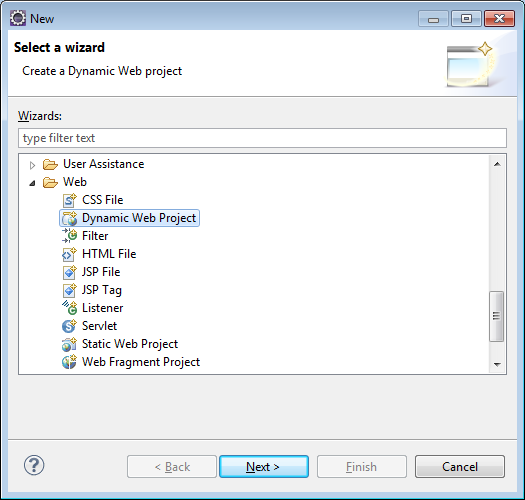
\includegraphics[scale=0.65]{./imagens/apendice_img1.png}}
  \caption[Exemplo de criação de um projeto Web no Eclipse]
          {Exemplo de criação de um projeto Web no Eclipse. \textbf{Fonte:} \cite{correa2003plantas}}
\label{fig:exemplo1}
\end{figure}

\par Perceba que o \LaTeX~faz a numeração automática das figuras e já adiciona na lista de figuras.

\par Agora a mesma imagem foi incluída, porém em escala menhor, conforme ilustra a Figura~\ref{fig:exemplo2}.:

\begin{figure}[h!]
  \centerline{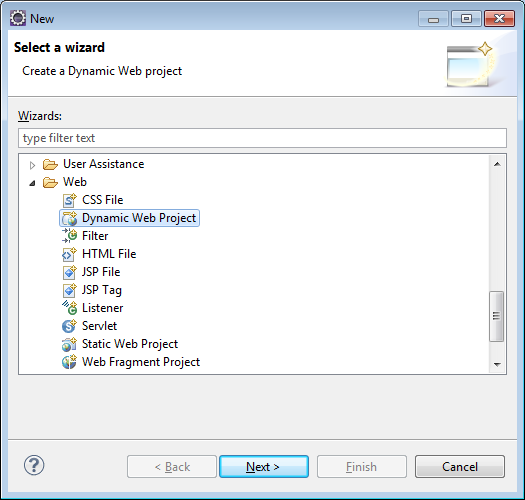
\includegraphics[scale=0.25]{./imagens/apendice_img1.png}}
  \caption[Mesma imagem em escala menor]
          {Mesma imagem em escala menor. \textbf{Fonte:} \cite{correa2003plantas}}
\label{fig:exemplo2}
\end{figure}

\chapter{QUADRO METODOLÓGICO}
\label{cap:quadroMetodologico}

\par Conteúdo do quadro metodológico. Perceba a forma que se coloca uma palavra entre aspas: o \LaTeX~oferece muita ``facilitade de formatação''.

Exemplo de código Java:

\begin{lstlisting} [style=custom_Java,caption={[Métodos da classe \texttt{FilmeBean}]{Métodos da classe \texttt{FilmeBean}. \textbf{Fonte:} Elaborado pelos autores.}}, label=fig:metodosclassebean] 	
	public FilmeBean(){  
       //...
   	}	
   	
	public void saveMovie(){
		setListActorSelected();		
		if(this.movieDAO.saveMovieGraph(this.movieTo)){
			FacesContext.getCurrentInstance().addMessage(null, 
			   new FacesMessage("Filme cadastrado com sucesso!")); 
		}else{
			//...
		}		
		this.limpaCampos();
	}
\end{lstlisting}

\par Agora será mostrado o exemplo do uso de fluxo de eventos apresentado no Quadro~\ref{quad:fluxo_evento_cadastro_filme}.

\begin{quadro}[h!]
  \begin{fluxoDeEventos}
  \addTitle{Cadastrar filme}
  \addrow{Ator principal}{Administrador}
  %\addrow{Ator secundário}{Sistema de cartão}
  \addrow{Pré-requisitos}{Estar logado no sistema}

  \startBasicFlow{Ator} {Sistema}
  \addItemOne{Seleciona menu cadastro}
  \addItemOne{Clica na opção cadastrar filme}
  \addItemTwo{Abre interface de cadastro de filme}
  \addItemOne{Preenche formulário}
  \addItemOne{Clica no botão salvar}
  \addItemTwo{Salva e informa sucesso no cadastro}

  \startAlternativeFlow{Fluxo alternativo 1}
  \addItemOne{No item 5, formulário não preenchido}
  \addItemTwo{Exibe mensagem de necessidade de preenchimento de formulário}

  \startAlternativeFlow{Fluxo alternativo 2}
  \addItemOne{No item 6, inserido filme já cadastrado}
  \addItemTwo{Informa mensagem de filme já cadastrado}
\end{fluxoDeEventos}

  \caption[Fluxo de eventos para cadastro de filme]
           {Fluxo de eventos para cadastro de filme. \textbf{Fonte:} Elaborado pelos autores}
  \label{quad:fluxo_evento_cadastro_filme}
\end{quadro}

\par Outro exemplo é ilustrado na Figura~\ref{fig:bluesky}. Neste caso um código XML foi embutido dentro de um ambiente de figura, para que este código seja incluído no índice de figuras adequadamente.
 
\begin{figure}[ht!]
  \begin{lstlisting} [style=custom_XML]
	...
	<context-param>
		<param-name>primefaces.THEME<\param-name>
		<param-value>bluesky<\param-value>
	<\context-param>
	...
  \end{lstlisting}
  \caption[Incluindo o tema \textit{BlueSky} ao contexto do projeto]
          {Incluíndo o tema \textit{BlueSky} ao contexto do projeto. \textbf{Fonte:} Elaborado pelos autores.}
  \label{fig:bluesky}
\end{figure}


\chapter{RESULTADOS} 

\par Aqui deve aparecer a descrição dos resultados obtidos.




\chapter{CONCLUSÃO} 

\par A conclusão deste trabalho é \ldots

\par Assim conclui-se que \ldots




\postextual %Início dos Elementos Pós-Textuais

%\citeoption{abnt-etal-cite=2}
\citeoption{ABNT-final}

\bibliography{biblio}               % insere as REFERÊNCIAS (arquivo biblio.bib)
\addcontentsline{toc}{chapter}{REFERÊNCIAS} % adiciona o título das referências no Sumário

\begin{apendicesenv}

%\apendicesname{APÊNDICES}
% Imprime uma página indicando o início dos apêndices
\partapendices*

\addcontentsline{toc}{chapter}{APÊNDICES}

\chapter*{Título do Apêndice I}
\label{apendice:1}

\par Aqui deve conter o texto do Apêndice~\ref{apendice:1}. Na Figura~\ref{fig:ap1:identificador} é ilustrada a primeira tela deste processo.
\captionsetup[figure]{list=no}
\begin{figure}[h!]
 \centerline{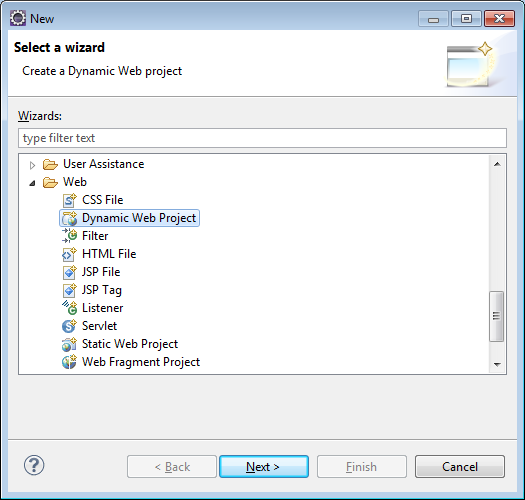
\includegraphics[scale=0.5]{./imagens/apendice_img1.png}}
 \caption[Outra imagem.]
           {Outra imagem. \textbf{Fonte:} Elaborado pelos autores}
  \label{fig:ap1:identificador}
\end{figure}

\par Após a seleção do tipo de projeto \ldots
\chapter*{Título do Apêndice 2}

\section*{Primeira seção do apêndice 2}

\par Neste apêndice é mostrado \ldots de acordo com a Figura~\ref{fig:ap2:identificador} é ilustrada a primeira tela deste processo.
\captionsetup[figure]{list=no}
\begin{figure}[h!]
 \centerline{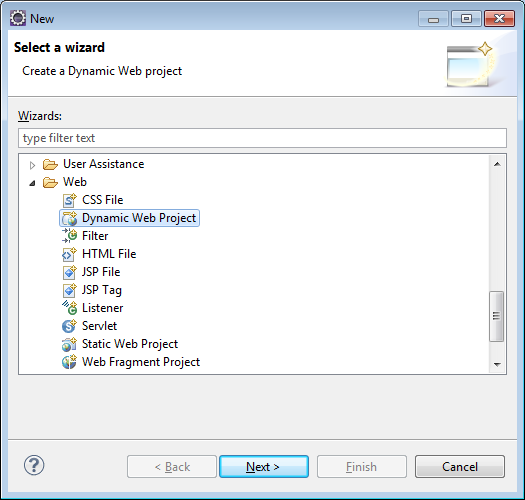
\includegraphics[scale=0.3]{./imagens/apendice_img1.png}}
 \caption[Outra imagem ainda.]
           {Outra imagem ainda. \textbf{Fonte:} Elaborado pelos autores}
  \label{fig:ap2:identificador}
\end{figure}

\section*{Segunda seção do apêndice 2}


\par Continuando \ldots na figura Figura~\ref{fig:xml_exemplo} é mostrado um exemplo de XML.

\begin{figure}[h!]
\begin{lstlisting}[style=custom_XML]
<project>
...
 <dependencies>
  ...
  <dependency>
   <groupId>org.neo4j</groupId>
   <artifactId>neo4j</artifactId>
   <version>1.9.4</version>
  </dependency>
  ...
 </dependencies>
 ...
</project>
\end{lstlisting}  
 \caption[Exemplo de código XML.]
           {Exemplo de código XML. \textbf{Fonte:} Elaborado pelos autores}
  \label{fig:xml_exemplo}
\end{figure}



\end{apendicesenv}
%\anexoname{ANEXOS}
%\begin{anexosenv}
%\partanexos
%\chapter*{ANEXO I}

\par Aqui deve aparecer o conteúdo do Anexo 1.
%\end{anexosenv}

\addcontentsline{toc}{chapter}{ANEXOS}

\chapter*{ANEXO I}

\par Aqui deve aparecer o conteúdo do Anexo 1.


\printindex

\end{document}